\chapter{Future improvement for Convolutional Neural Network ID}
\label{Adx3}
The developed CNN ID algorithm shows a better performance over the cut-based algorithm and seems to be promising, while the algorithms still not the state of art and several improvement are required to improve its performance in the future. This chapter discusses the ideas I have to improve the CNN algorithm.

\section{Low efficiency at high $\eta$}
\label{Adx3:Eta}

As discussed in section \ref{gamma:CNN:Zllg}, CNN performance degrade significantly for low \pT and high $\eta$ photons. This is explained with the fact that low energy photons deposit a large fraction of their energy in the first EM sampling, and given the size of the first sampling images specially at high $\eta$, the CNN efficiency for those photons is very low. This is illustrated in Figure \ref{fig:Adx3:Eta}. Note that the training does not take any information about the direction of the photons.
\begin{figure}[htbp]
    \centering
    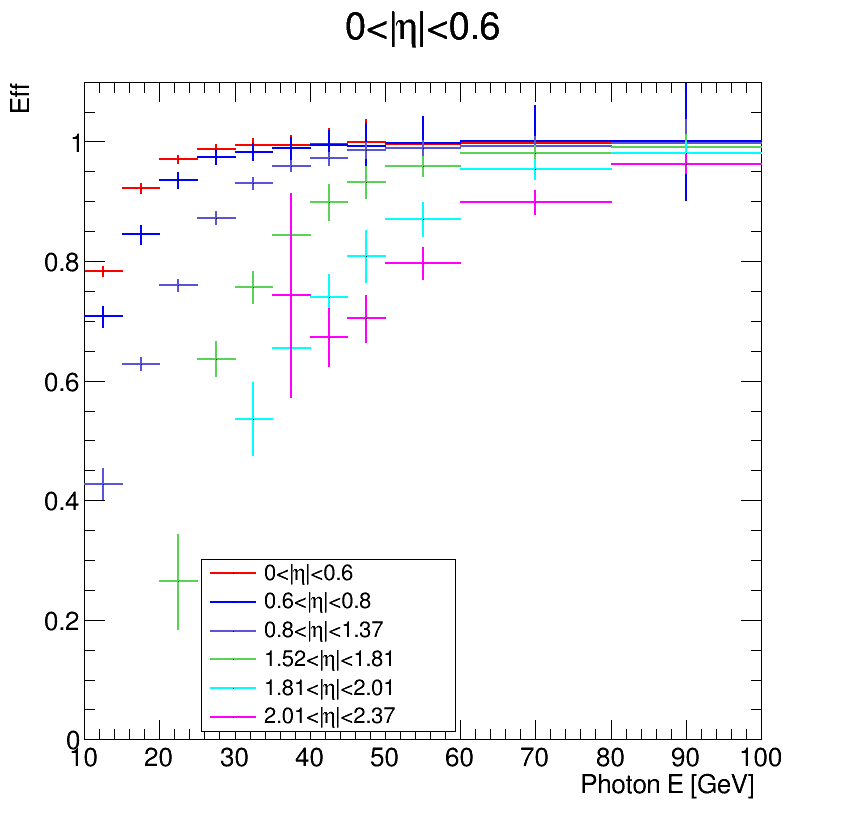
\includegraphics[width=0.6\textwidth]{Adx/Adx3/Img/Eff_vs_Energy.png}
    \begin{tcolorbox}[colback=black!5!white,colframe=white!75!black]
    \caption{CNN efficiency as a function of photon transvers energy for different $\eta$ regions. }
    \label{fig:Adx3:Eta}
    \end{tcolorbox}
    
\end{figure}

There was several discussion on how to include $\eta$ as an input variable to the CNN, while the CNN should not take $\eta$ as a discriminant between the signal and background. A reweighting technique to re-weight the $\eta$ distribution to be similar between signal and background can be used in this case. Personally, developing a specific convolution layer which take into account the direction of the photon is the best solution, but technically complicated. Such convolution layer will be able to to define the size of the convolutional filter needed to extract the shower form first layer images for given $\eta$ region. \\

\section{Multi-Task Cascade Convolutional Network (MTCNN)}

The Multi-Task Cascade Convolutional Network (MTCCN) is an alternative, much easier, solution to take photon direction into account. The MTCCN is a technique used for face detection and alignment to detect objects in large images without losing efficiency. The MTCCN consists mainly of three stage. In the first stage, it produces candidate windows quickly through a shallow CNN. Then,  it  refines the windows to reject a large number of non-photon windows through a more complex CNN. Finally, it uses a more powerful CNN to refine the result and output positions. This technique will be able to define the convolutional frame for each photon, in this way the network will be able to catch the shower of small images without be affected by the whitens in the image. The MTCCN is able to work with any size of image and benign unaffected, thus the motivation to be used with topological cluster as well. The fact that MTCCN is able to define its convolutional filter for each photon to extract the shower, makes it a good candidate to handle photon isolation in order to reduce closure uncertainties. Figure \ref{fig:Adx3:MTCCN} shows an illustration of the MTCCN applied to a topological cluster. The green rectangle shows the global image size, the dashed rectangles show the candidate windows defined by the CNN at the first stage, the solid rectangle is the windows photons defined at stage 2. Dots are the position used to describe the shower of the photon in more details. 
\begin{figure}[htbp]
    \centering
    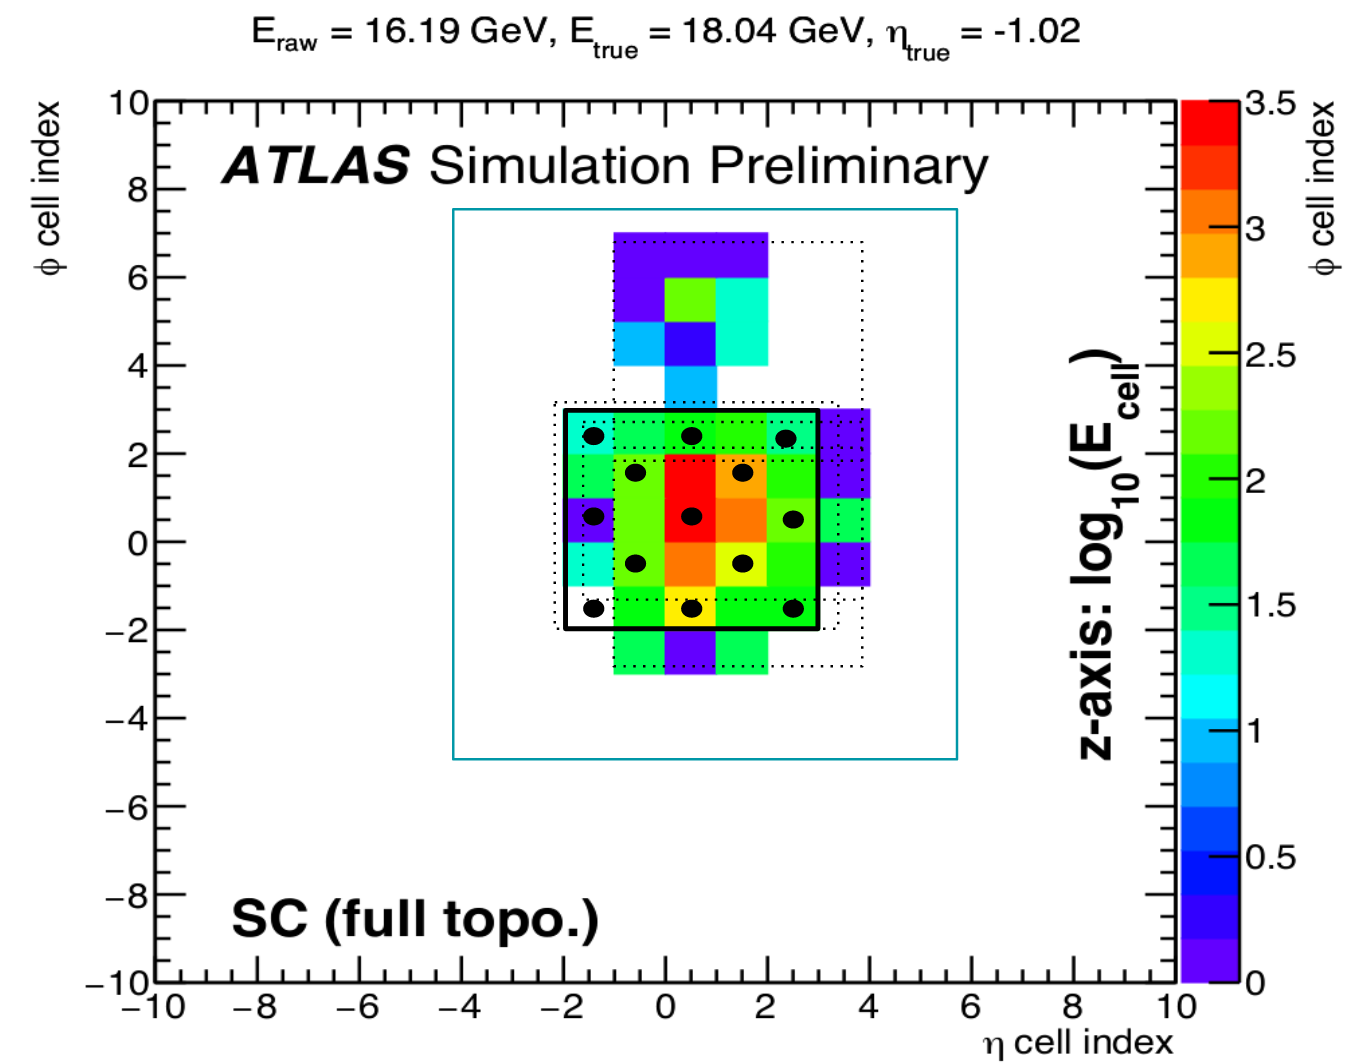
\includegraphics[width=0.6\textwidth]{Adx/Adx3/Img/MTCCN.png}
    \caption{Schema for MTCCN applied to a topological cluster.}
    \label{fig:Adx3:MTCCN}
\end{figure}

\section{Pile-Up dependency}
The second issue of the CNN is the pile-up dependency which makes the efficiency decreases for high pile-up events. This effect will be critical for HL-LHC. In medicine area, machine learning is used to extract noise from medical images using Auto-Encoder technique. The Auto-Encoder is used to learn the latent representation of the image which is used later to generate the image without noise as schematized in Figure \ref{fig:Adx3:AutoEncoder}.

\begin{figure}[H]
    \centering
    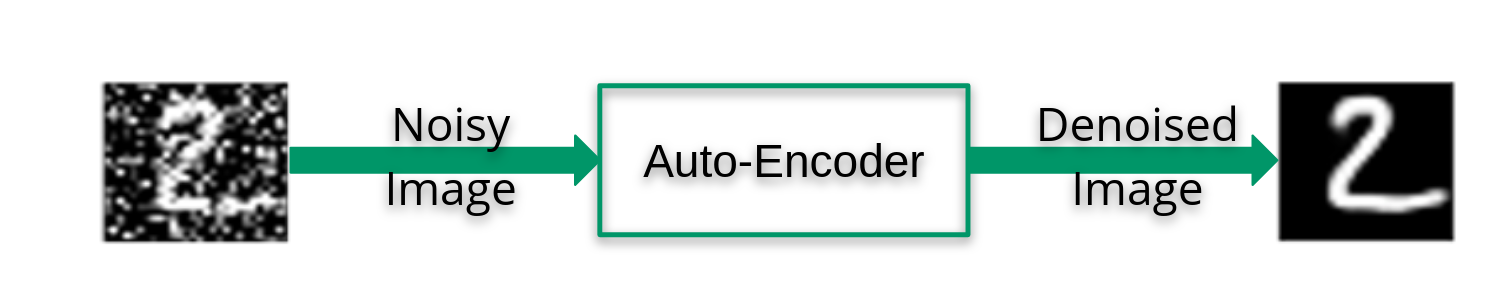
\includegraphics[width=0.85\textwidth]{Adx/Adx3/Img/AutoEncoder.png}
    \caption{Image de-noising with AutoEncoder}
    \label{fig:Adx3:AutoEncoder}
\end{figure}

The same idea can be used to reduce pile-up from shower images. An auto-encoder can be trained for each layer using two exact generated sample one with pile-up and one without pile-up, the auto-encoder is trained to generate the the non-pile images from the one with pile-up. The produced images are then passed to the CNN for classification task. The new Pile-Up Auto-Encoder Denoising (PAED) algorithm to remove pile-up is shown in Figure \ref{fig:Adx3:PAED}.

\begin{figure}[htbp]
    \centering
    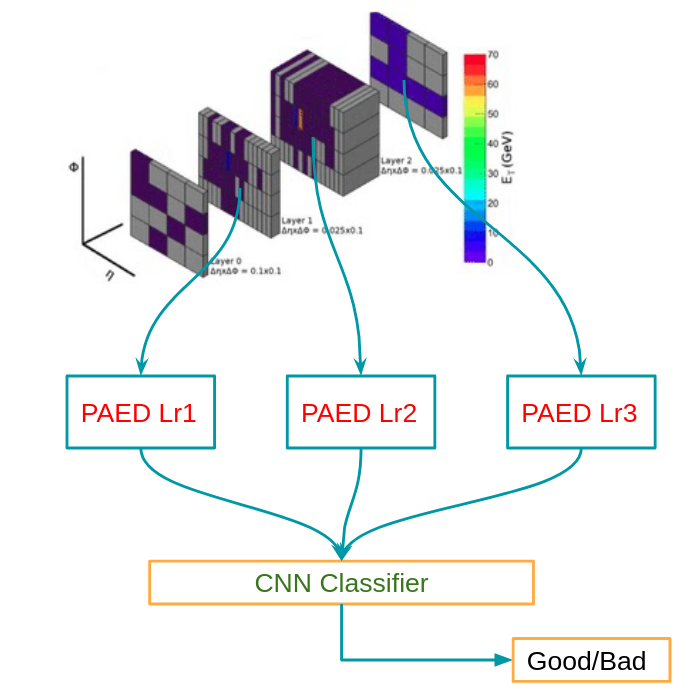
\includegraphics[width=0.55\textwidth]{Adx/Adx3/Img/PAED.png}
    \begin{tcolorbox}[colback=black!5!white,colframe=white!75!black]
    \caption{CNN classifier with PAED schema.}
    \label{fig:Adx3:PAED}
    \end{tcolorbox}
    
\end{figure}